\documentclass[12pt]{article}
\usepackage{amsthm,amssymb,amsmath,amsfonts}
\usepackage[a4paper, top=25mm, bottom=30mm, left=25mm, right=25mm]{geometry}
\usepackage[pagebackref=false,colorlinks,linkcolor=black,citecolor=black]{hyperref}
\usepackage[nameinlink]{cleveref}
 \AtBeginDocument{%
    \crefname{equation}{برابری}{equations}%
    \crefname{chapter}{فصل}{chapters}%
    \crefname{section}{بخش}{sections}%
    \crefname{appendix}{پیوست}{appendices}%
    \crefname{enumi}{مورد}{items}%
    \crefname{footnote}{زیرنویس}{footnotes}%
    \crefname{figure}{شکل}{figures}%
    \crefname{table}{جدول}{tables}%
    \crefname{theorem}{قضیه}{theorems}%
    \crefname{lemma}{لم}{lemmas}%
    \crefname{corollary}{نتیجه}{corollaries}%
    \crefname{proposition}{گزاره}{propositions}%
    \crefname{definition}{تعریف}{definitions}%
    \crefname{result}{نتیجه}{results}%
    \crefname{example}{مثال}{examples}%
    \crefname{remark}{نکته}{remarks}%
    \crefname{note}{یادداشت}{notes}%
    \crefname{observation}{مشاهده}{observations}%
    \crefname{algorithm}{الگوریتم}{algorithms}%
    \crefname{cproof}{برهان}{cproofs}%
}

\usepackage{tikz}
\usepackage{graphicx}
\usepackage{booktabs}
\usepackage{color}
\usepackage{graphicx}
\usepackage{subcaption}

\usepackage{setspace}
\doublespacing

\usepackage{titletoc}
\usepackage{tocloft}
\usepackage{enumitem}
\usepackage{amsmath, amssymb}
\usepackage{algorithm}
\usepackage[noend]{algorithmic}
\renewcommand{\algorithmicrequire}{\textbf{Input:}}
\renewcommand{\algorithmicensure}{\textbf{Output:}}

\usepackage{tabularx}
\makeatletter
\newcommand{\multiline}[1]{%
  \begin{tabularx}{\dimexpr\linewidth-\ALG@thistlm}[t]{@{}X@{}}
    #1
  \end{tabularx}
}
\makeatother

\usepackage{float}
\usepackage{verbatim}
\makeindex
\usepackage{sectsty}
\usepackage{xepersian}
\SepMark{-}
\settextfont[Scale=1.2,Path=fonts/,BoldFont=B Nazanin Bold.ttf]{B Nazanin.ttf}
\setlatintextfont{Times New Roman}
\renewcommand{\labelitemi}{$\bullet$}

\theoremstyle{definition}
\newtheorem{definition}{تعریف}[section]
\newtheorem{remark}[definition]{نکته}
\newtheorem{note}[definition]{یادداشت}
\newtheorem{example}[definition]{نمونه}
\newtheorem{question}[definition]{سوال}
\newtheorem{remember}[definition]{یاداوری}
\newtheorem{observation}[definition]{مشاهده}
\theoremstyle{theorem}
\newtheorem{theorem}[definition]{قضیه}
\newtheorem{lemma}[definition]{لم}
\newtheorem{proposition}[definition]{گزاره}
\newtheorem{corollary}[definition]{نتیجه}
\newtheorem*{cproof}{برهان}




\begin{document}
\fontsize{12pt}{14pt}\selectfont

\begin{minipage}{0.1\textwidth}

\includegraphics[width=3cm]{etc/IUST}
\end{minipage}%
\hfill%
\begin{minipage}{0.6\textwidth}\centering
\fontsize{13pt}{13pt}\selectfont
به‌ نام خدا \\
\textbf{درس یادگیری عمیق} \\
\textbf{تمرین سری ششم}\\
استاد درس : دکتر محمدرضا محمدی \\
دستیاران :  مهدی خورشا، سید محمد موسوی،\\ امیرحسین نمازی
\\
\vspace{0.25cm}
\begingroup
\fontsize{11pt}{11pt}\selectfont
دانشگاه علم و صنعت ایران، دانشکده مهندسی کامپیوتر \\
نیمسال دوم تحصیلی 1403 - 1404 \\
\endgroup
\end{minipage}%
\hfill%
\begin{minipage}{0.1\textwidth}

\end{minipage}

\vspace{0.5cm}

\noindent\rule{\textwidth}{1pt}

\centering {\fontsize{18}{22}\selectfont \textbf{مهلت تحویل : 1404/05/05 }}\\
{\fontsize{14}{22}\selectfont \textbf{لطفا به نکات موجود در سند قوانین انجام و تحویل تمرین ها دقت فرمایید. }}

\begin{enumerate}

    \section*{سوالات تئوری}
    \item 
\includegraphics[width=1cm]{figs/Forbidden_AI.jpg}
    روش‌های پیشرفته‌ی یادگیری ماشین خودکار مانند جستجوی معماری عصبی (\lr{NAS}) و \lr{AutoAugment}  برای خودکارسازی جنبه‌های پیچیده طراحی مدل توسعه یافته‌اند. اصول اصلی این روش‌ها را توضیح دهید و موارد زیر را بررسی کنید. برای هریک از ۲ روش ذکر شده، موارد ذیل را به صورت جداگانه مورد بحث قرار دهید:(۲۰ نمره)
    
    \begin{enumerate}
        \item نحوه تعریف مسئله‌ی خودکارسازی توسط هر تکنیک
        \item سازوکارها یا ساختارهای کنترلی مورد استفاده (مثل \lr{Controller-Trainer}، \lr{sub-policies})
        \item چالش‌های مرتبط با پیچیدگی فضای جستجو و هزینه محاسباتی
        \item نقش یادگیری تقویتی (\lr{RL})، بهینه‌سازی بیزی و تطابق چگالی در حل این چالش‌ها
        \item ذکر نمونه‌ها یا نسخه‌های خاص هر روش (در صورت وجود)
    \end{enumerate}

     
    \item 
\includegraphics[width=1cm]{figs/Forbidden_AI.jpg}
    \begin{enumerate}
            \item ماتریس \lr{W} زیر را در نظر بگیرید. ابتدا تعریف کنید که مرتبه (\lr{rank}) یک ماتریس چیست و چه مفهومی دارد سپس مرتبه ماتریس \lr{W} را به صورت دستی محاسبه کنید. در ادامه ماتریس \lr{W} را به دو ماتریس تجزیه کنید به گونه ای که حاصل‌ضرب آن‌ها برابر با \lr{W}  باشد ( از مرتبه ماتریس استفاده کنید). در نهایت محاسبه کنید که تعداد پارامترها در این تجزیه، نسبت به تعداد پارامترهای اولیه ماتریس \lr{W}، چقدر کاهش پیدا کرده است. تاثیر مرتبه ماتریس را در تعداد پارامترها بررسی کنید. ( 5 نمره) 
        $$
            W=\left[\begin{array}{ccccc}
            1 & 3 & 0 & 2 & 3 \\
            0 & 1 & -2 & 1 & 2 \\
            2 & 5 & 1 & 3 & 4 \\
            1 & 2 & 1 & 1 & 1 \\
            3 & 7 & 2 & 4 & 5
            \end{array}\right]
        $$
        \item )  با توجه به مقاله \lr{LoRA} به سوالات زیر پاسخ دهید.  مدل پیش‌آموزش دیده \lr{BERT} با مشخصات زیر داده شده است:\\
        \lr{Model dimension: 1024, number of blocks: 24, number of attention heads: 16, vocabulary size: 30000, Rank r of LoRA: 16}\\
        
        هدف ما آموزش دقیق این مدل پیش‌آموخته بر روی دو تسک \lr{Question Answering} و \lr{Sentiment Analysis} می‌باشد.
        تعداد پارامترهای قابل آموزش و تعداد پارامترهای ذخیره‌سازی برای \lr{inference} را در دو حالت زیر بدست آورید: ( ۵ نمره) 
        \begin{itemize}
            \item آموزش با \lr{LoRA} 
            \item تنظیم دقیق معمولی ( بدون \lr{LoRA}) 
        \end{itemize}
        توجه: فقط پارامترهای بخش \lr{attention} را در نظر بگیرید.
        \item با توجه به مقاله \lr{LoRA}، توضیح دهید که چه میزان تأخیر (\lr{latency}) در مرحله \lr{inference} به مدل اضافه می‌شود. درستی جواب خود را اثبات کنید. همچنین بررسی کنید که مرتبه (\lr{rank}) در کدام بخش از شبکه تاثیرگذار است. ( ۵ نمره)
        \item در تصویر زیر، یک معماری آداپتور برای شبکه‌های کانولوشنی نمایش داده شده است که ماژول "آداپتور" به‌ طور موازی با یک بلوک کانولوشنی (\lr{ConvBlock}) عمل می‌کند و خروجی آن به خروجی بلوک کانولوشنی اضافه می‌شود. در تصویر بعدی، هیستوگرام‌های \lr{feature map} های خروجی هر دو ماژول نشان داده شده‌اند. این هیستوگرام‌ها چه تفاوت‌هایی دارند و دلیل این تفاوت‌ها چیست؟ این تفاوت‌ها چه مشکلاتی می‌توانند ایجاد کنند و برای رفع این مشکلات چه راه‌حل‌هایی پیشنهاد می‌دهید؟ ( ۵ نمره)
        \begin{figure}[h]
        \centering
        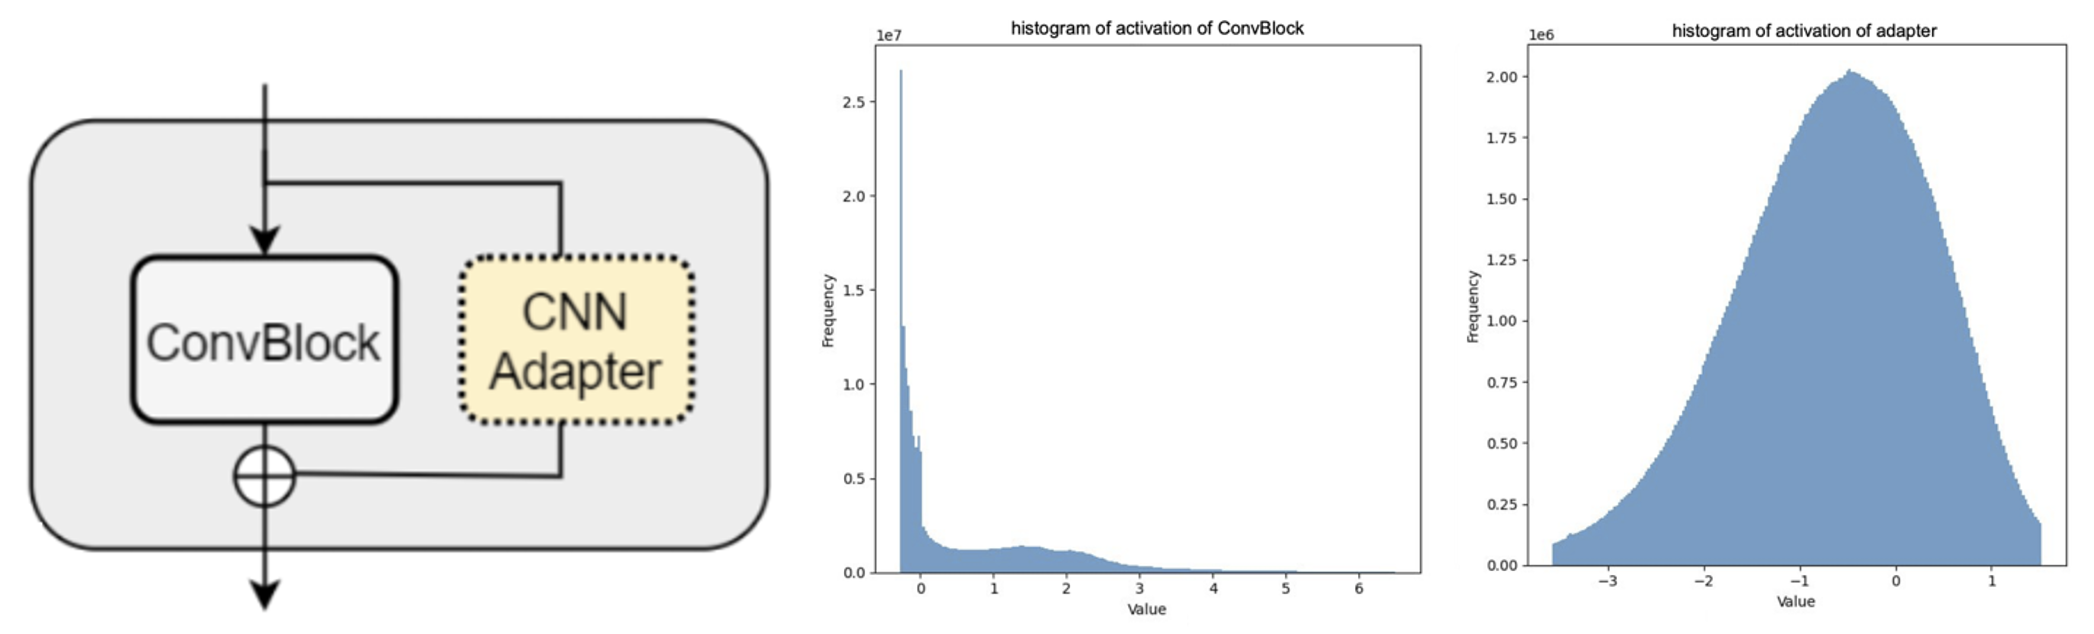
\includegraphics[width=\textwidth]{figs/Q2_4.png}
        \label{fig:q4}  
    \end{figure}
    \end{enumerate}

    \item 
\includegraphics[width=1cm]{figs/Allowed_recommended.jpg}فرض کنید در حال کار روی یک پروژه طبقه‌بندی تصاویر پزشکی برای تشخیص یک بیماری نادر هستید. شما با دو چالش اصلی روبرو هستید:
        \begin{itemize}
            \item تعداد تصاویر برچسب‌خورده بسیار محدود است.
            \item مشخص نیست که چه نوع معماری شبکه‌ای برای این داده‌های خاص بهترین عملکرد را خواهد داشت.
        \end{itemize}
        با الهام از روش‌های معرفی شده در درس یک راهبرد\LTRfootnote{Strategy} جامع برای ساخت یک مدل طبقه‌بندی با کارایی بالا پیشنهاد دهید. در پاسخ خود به موارد زیر بپردازید(۱۵ نمره):
        \begin{itemize}
            \item برای انتخاب معماری، کدام رویکرد را انتخاب می‌کنید؟دلیل انتخاب خود را توضیح دهید.
            \item مزایا و معایب انتخاب شما در این شرایط خاص چیست؟
            \item چالش‌های اصلی در راهبرد پیشنهادی شما کدامند؟
        \end{itemize}
        
    \item 
\includegraphics[width=1cm]{figs/Allowed_recommended.jpg}\lr{Fast AutoAugment} به عنوان یک راهکار برای رفع مشکل اصلی \lr{AutoAugment}، یعنی هزینه محاسباتی بالا، معرفی شده است. با توجه به الگوریتم و توضیحات ارائه شده در درس، به سوالات زیر پاسخ دهید(۱۵ نمره):
    \begin{enumerate}
        \item ایده کلیدی پشت \lr{Fast AutoAugment} که آن را سریع‌تر می‌کند، چیست؟ مفهوم 
تطابق چگالی\LTRfootnote{Density Matching} را توضیح دهید.
        \item استراتژی تقسیم داده‌ها به \lr{K-fold} و استفاده از مجموعه‌های $D_{\mathcal{A}}^{(k)}, D_{\mathcal{M}}^{(k)}$ چگونه به کاهش هزینه محاسباتی کمک می‌کند؟
        \item با استفاده از جدول مقایسه هزینه محاسباتی ، تفاوت سرعت این روش با \lr{AutoAugment} را برای مجموعه داده \lr{ImageNet} به صورت کمی بیان کرده و اهمیت این بهبود را تحلیل کنید.
    \end{enumerate}


   
    \section*{سوالات عملی} 
    \item 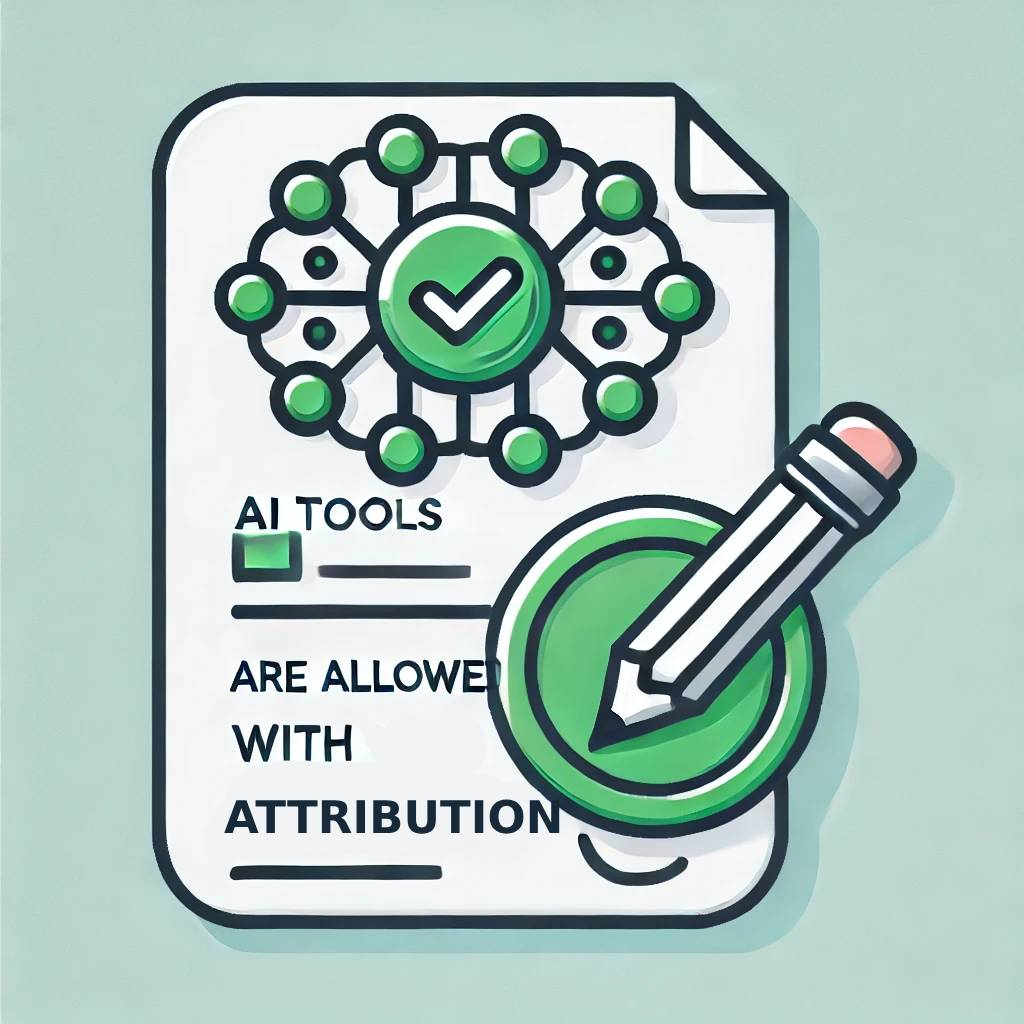
\includegraphics[width=1cm]{figs/Allowed_with_contributino.jpg}
    در این تمرین، قصد داریم فرآیند بهینه‌سازی یک شبکه عصبی را به صورت عملی تجربه کنیم. این فرآیند با ساخت یک مدل پایه  آغاز شده و با پیاده‌سازی و مقایسه طیف وسیعی از تکنیک‌های بهینه‌سازی هایپرپارامتر، از روش‌های کلاسیک مانند جستجوی شبکه‌ای تا الگوریتم‌های پیشرفته مانند \lr{Optuna} با قابلیت هرس کردن و الگوریتم ژنتیک، ادامه می‌یابد.
    وظیفه اصلی شما، تکمیل بخش‌های مشخص‌شده در نوت‌بوک \lr{HyperparameterOptimization.ipynb} است. در نهایت، از شما خواسته می‌شود تا نتایج روش‌های مختلف را تحلیل کرده و کارایی و عملکرد آن‌ها را با یکدیگر مقایسه نمایید(۳۰ نمره).




\end{enumerate}



\end{document}


